\section{Động tác xoa bóp bấm huyệt}

\subsection{Thủ thuật tác động lên da}

\begin{longtblr}[
    caption = {Thủ thuật tác động lên da},
]{
    width = \textwidth,
    colspec = {|X[1,c]|X[1,l]|X[2.5,l]|X[2.5,l]|X[2.5,l]|X[2.5,l]|},
    % hlines,
    rowhead = 1,
}
    \hline
    ID & Thủ thuật & Cơ quan thực hiện & Yêu cầu & Vùng tác động & Quỹ đạo \\ \hline
    1 & \xoa & {%
        1. Gốc bàn tay \newline
        2. Ô mô út \newline
        3. Ngón tay cái
    } & {%
        1. Chậm \newline
        2. Nhẹ
    } & {%
        1. Bụng
    } & {%
        1. Đường tròn
    }
    \\ \hline
    2 & \xat & {%
        1. Gốc bàn tay \newline
        2. Mô ngón út \newline
        3. Ngón tay cái
    } & {%
        1. Nhanh \newline
        2. Có lực
    } & {%      
    } & {%
        1. Lên xuống \newline
        2. Phải sang trái
    }
    \\ \hline
    3 & \miet & {%
        1. Ngón tay cái
    } & {
        1. Chậm \newline
        2. Có lực
    } & {%
        1. Bụng \newline
        2. Đầu
    } & {%
        1. Trên xuống \newline
        2. Dưới lên \newline
        3. Phải sang trái \newline
        4. Trái sang phải
    }
    \\ \hline
    4 & \phanhop & {%
        1. Ngón tay cái \newline
        2. Đầu của ba ngón: 2, 3, 4 \newline
        3. Ô mô út
    } & {%
        1. Kéo đều ra hai bên (phân) \newline
        2. Từ hai bên kéo vào (hợp)
    } & {%
        1. Trán \newline
        2. Đầu \newline
        3. Mặt \newline
        4. Bụng \newline
        5. Lưng \newline
        6. Ngực
    } & {%
        1. Phân hợp ngang \newline
        2. Phân hợp v
    }
    \\ \hline
    5 & \veo & {%
        1. Đầu ngón tay cái và ngón tay trỏ
    } & {%
        1. Kéo da \newline
        2. Da luôn bị cuộn ở giữa các ngón tay
    } & {%
        1. Lưng \newline
        2. Trán
    } & {%
        1. Tịnh tiến
    }
    \\ \hline
    6 & \vo & {%
        1. Bàn tay
    } & {%
        1. Khum bàn tay (lòng bàn tay lõm) \newline
        2. Phát nhẹ tăng dần
    } & {
        1. Vai \newline
        2. Lưng \newline
        3. Tứ chi
    } & {%
        1. Tịnh tiến
    }
    \\ \hline
\end{longtblr}


\subsection{Thủ thuật tác động lên cơ}

\begin{longtblr}[
    caption = {Thủ thuật tác động lên cơ},
]{
    width = \textwidth,
    colspec = {|X[1,c]|X[1,l]|X[2.5,l]|X[2.5,l]|X[2.5,l]|X[2.5,l]|},
    % hlines,
    rowhead = 1,
}
    \hline
    ID & Thủ thuật & Cơ quan thực hiện & Yêu cầu & Vùng tác động & Quỹ đạo
    \\ \hline
    1 & \acday & {%
    1. Mô út \newline
    2. Gốc bàn tay
    } & {%
    1. Khoan thai \newline
    2. Ấn vừa với sức chịu đựng của người bệnh. 
    } & {%
    } & {%
    1. Đường tròn \newline
    }
    \\ \hline
    2 & \dam & {%
    } & {%
    } & {%
    } & {%
    }
    \\ \hline
    3 & \chat & {%
    1. Bàn tay \newline
    2. Cổ tay
    } & {%
    1. Cổ tay mềm dẻo \newline
    2. Tiếng kêu của bàn tay
    } & {%
    1. Cổ gáy \newline
    2. Vai \newline
    3. Lưng \newline
    4. Mông
    } & {%
    }
    \\ \hline
    4 & \lan & {%
    1. Mặt bên ngoài của mô út \newline
    2. Mặt ngoài ngón út
    } & {%
    1. Khéo léo vận động khớp cổ tay \newline
    2. Có lực điệu \newline
    3. Có sức ép nhất định
    } & {%
    1. Lưng \newline
    2. Vai \newline
    3. Mông \newline
    4. Tứ chi \newline
    } & {
    }
    \\ \hline
    5 & \bop & {%
    1. Ngón một và ngón hai \newline
    2. 5 ngón
    } & {%
    1. Kéo vùng cơ của người bệnh. \newline
    2. Vừa phải tránh đau đớn.
    } & {%
    1. Cổ \newline
    2. Gáy \newline
    3. Vai \newline
    4. Nách \newline
    5. Tứ chi
    } & {%
    }
    \\ \hline
    6 & Vờn & {%
    1. Hai bàn tay
    } & {%
    1. Hai bàn tay bao lấy vị trí nhất định. \newline
    2. Da thịt chuyển động theo \newline
    3. Nhẹ nhàng
    } & {%
    } & {%
    1. Ngược chiều \newline
    2. Trên xuống \newline
    3. Dưới lên
    }
    \\ \hline
\end{longtblr}

\subsection{Vận động}
\subsubsection{Vận động khớp cổ}

\begin{longtblr}[
    caption = {Vận động khớp cổ},
]{
    width = \textwidth,
    colspec = {|X[1,c]|X[1,c]|X[1,c]|X[9,l]|},
    % hlines,
    rowhead = 1,
}
    \hline
     STT & Động tác & Số lượt & Ghi chú
     \\ \hline
     1 & Cúi & 3 & {
        \cui
        \newline
        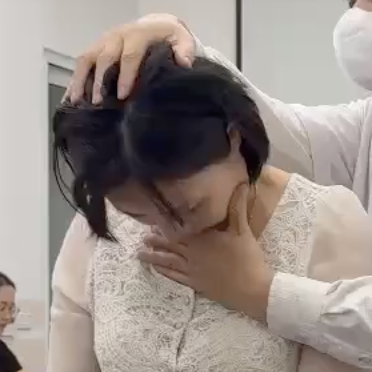
\includegraphics[width=0.48\linewidth]{cui_01.png}
        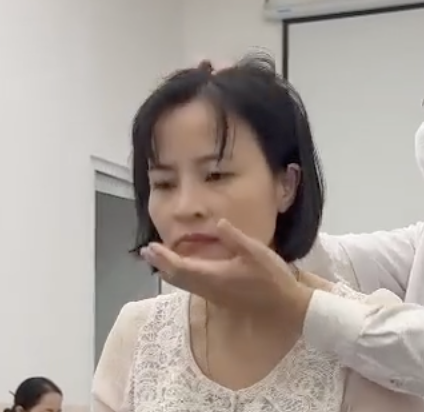
\includegraphics[width=0.48\linewidth]{cui_02.png}
        \newline
        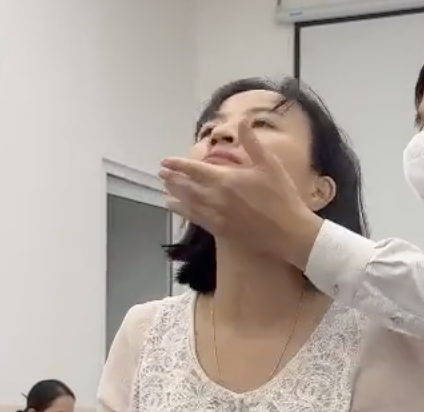
\includegraphics[width=0.48\linewidth]{cui_03.png}
        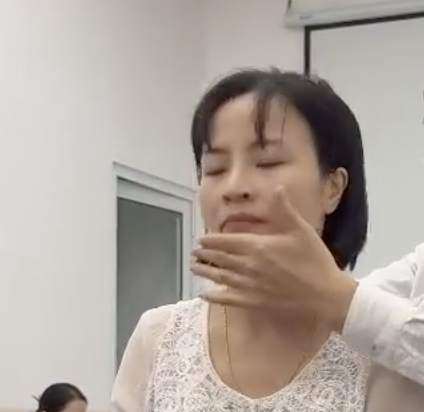
\includegraphics[width=0.48\linewidth]{cui_04.png}
     }
    \\ \hline
    2 & Ngửa & 3 & {
        \ngua (Sau khi đẩy trán thì bỏ tay ra để cổ duỗi thẳng tự nhiên)
        \newline
        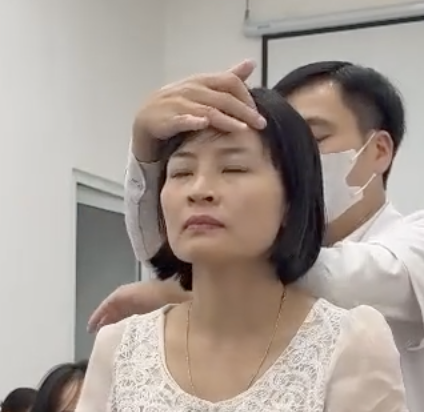
\includegraphics[width=0.48\linewidth]{ngua_01.png}
        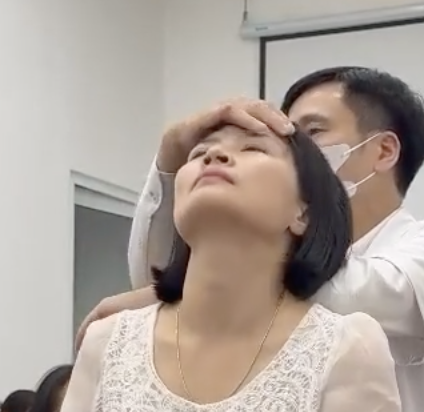
\includegraphics[width=0.48\linewidth]{ngua_02.png}
     }
    \\ \hline
    3 & Nghiêng trái & 3 & {
        \nhiengtrai
        \newline
        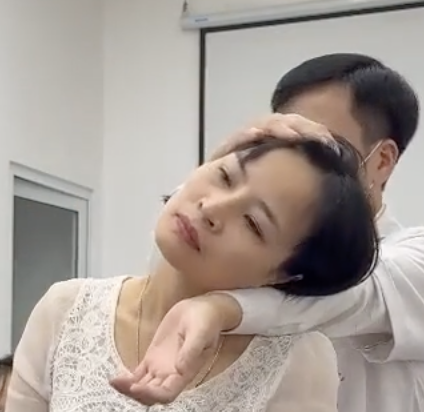
\includegraphics[width=\linewidth]{nghientrai_01.png}
    }
    \\ \hline
    4 & Nghiêng phải & 3 &{
        \nhiengphai
        \newline
        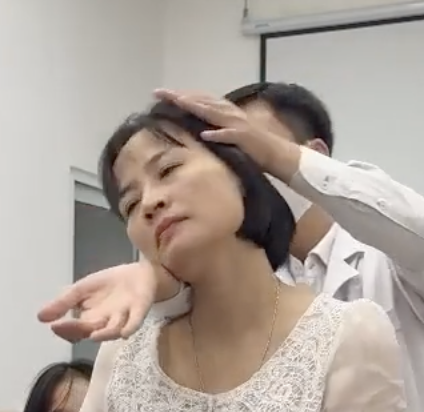
\includegraphics[width=\linewidth]{nghieng_phai_01.png}
    }
    \\ \hline
    4 & Xoay trái & 3 & {
        \xoaytrai: Tới tầm là thôi. Căng tay là dừng 
        \newline
        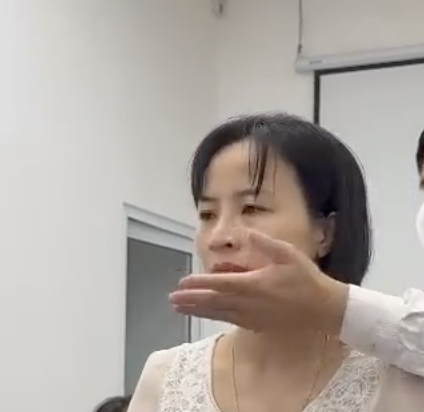
\includegraphics[width=0.48\linewidth]{xoay_trai_01.png}
        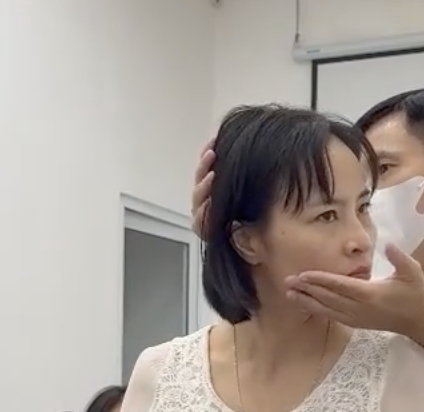
\includegraphics[width=0.48\linewidth]{xoay_trai_02.png}
        \newline
        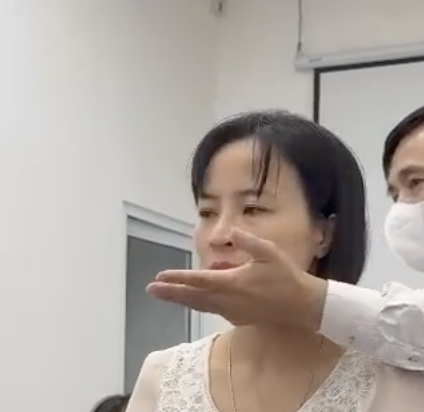
\includegraphics[width=\linewidth]{xoay_trai_03.png}
     }
     \\ \hline
    5 & Xoay phải & 3 & {
        \xoayphai: Tới tầm là thôi. Căng tay là dừng
        \newline
        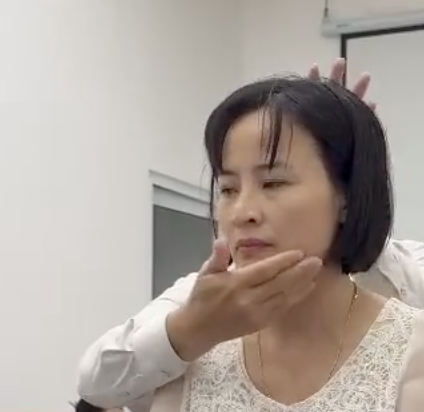
\includegraphics[width=0.48\linewidth]{xoay_phai_01.png}
        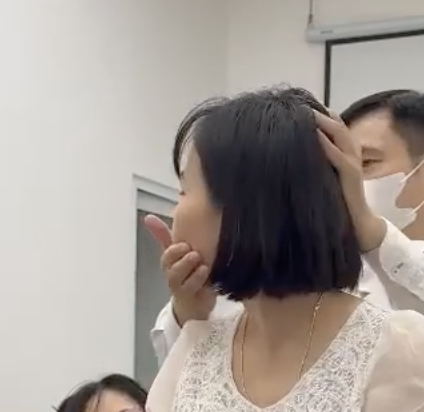
\includegraphics[width=0.48\linewidth]{xoay_phai_02.png}
        \newline
        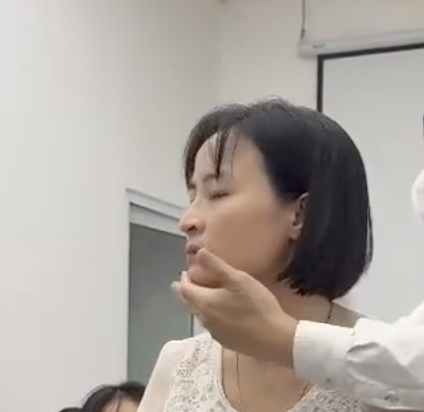
\includegraphics[width=0.48\linewidth]{xoay_phai_03.png}
        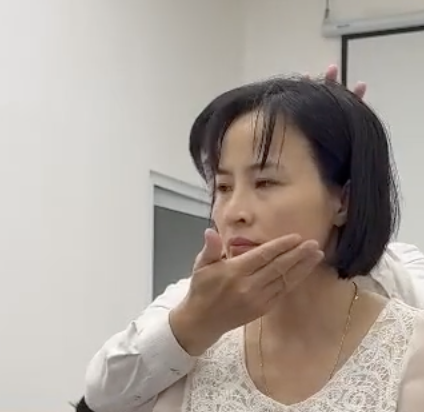
\includegraphics[width=0.48\linewidth]{xoay_phai_04.png}
     }
     \\ \hline
     6 & Xoay hỗn hợp & 3 & {
        \xoayhonhop \newline
        1. Một tay đỡ cằm \newline
        2. Một tay đỡ chẩm \newline
        3. Xoay
        \newline
        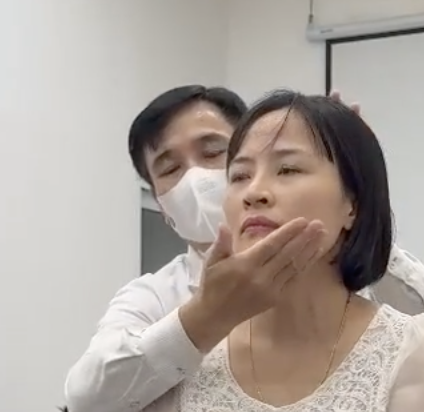
\includegraphics[width=0.48\linewidth]{xoay_hon_hop_01.png}
        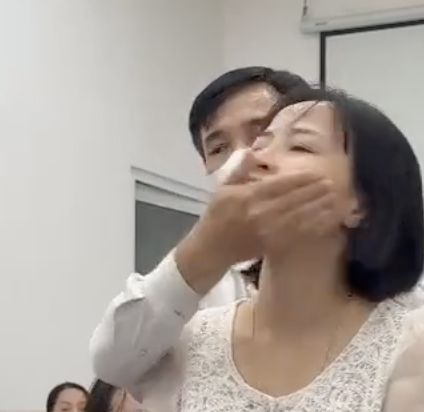
\includegraphics[width=0.48\linewidth]{xoay_hon_hop_02.png}
     }
     \\ \hline
\end{longtblr}

\subsubsection{Vận động khớp tay}

\textbf{Vận động khớp vai}

\begin{longtblr}[
    caption = {Vận động khớp vai},
]{
    width = \textwidth,
    colspec = {|X[1,c]|X[1,c]|X[1,c]|X[9,l]|},
    % hlines,
    rowhead = 1,
}
    \hline
    STT & Tên & Số lần & Ghi chú
    \\ \hline
    1 & Xoay vòng nhỏ & & {%
        \hypertarget{target:xoay_vong_nho}{\textbf{Xoay vòng nhỏ:}}

        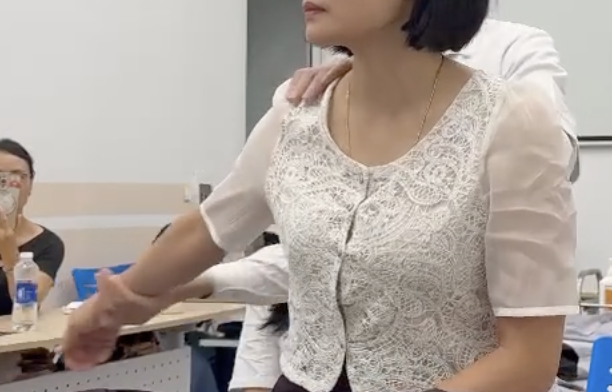
\includegraphics[width=0.48\linewidth]{van_dong_kho_vai_02.png}
        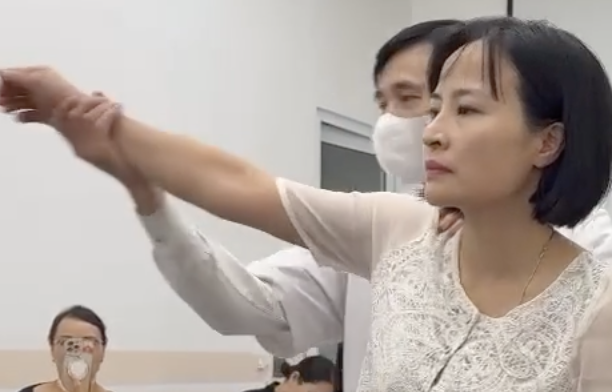
\includegraphics[width=0.48\linewidth]{van_dong_khop_vai_02.png}
    }
    \\ \hline
    2 & Xoay vòng lớn & & {%
        \hypertarget{target:xoay_vong_lon}{\textbf{Xoay vòng lớn:}} bao gồm xoay xuôi và xoay ngược

        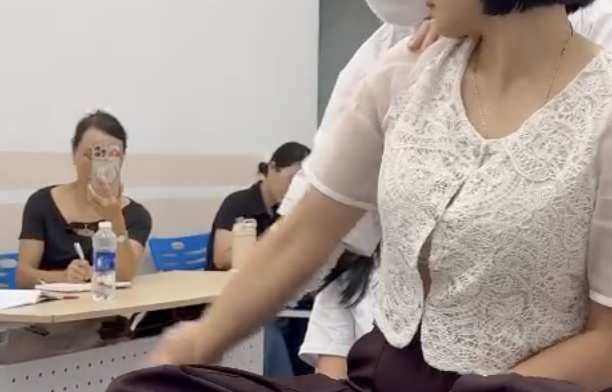
\includegraphics[width=0.48\linewidth]{xoay_vong_lon_01.png}
        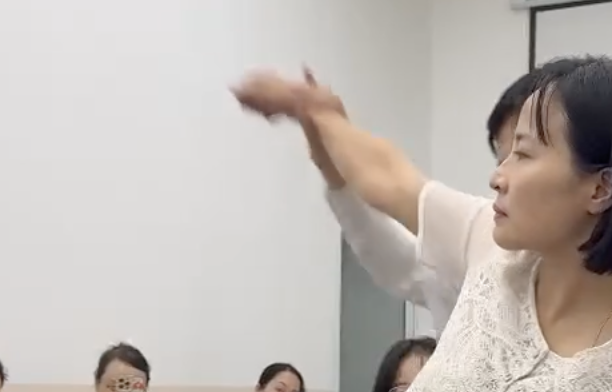
\includegraphics[width=0.48\linewidth]{xoay_khop_vai_02.png}
    }
    \\ \hline
    3 & Xoay mở khớp vai & & {%
        \hypertarget{target:xoay_mo_khop_vai}{\textbf{Xoay mở khớp vai:}} Lựa tới tầm căng cơ

        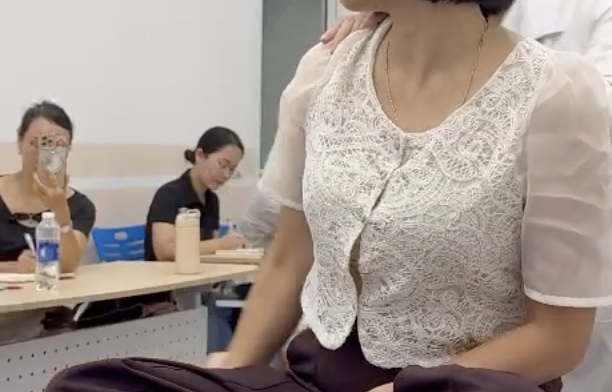
\includegraphics[width=0.48\linewidth]{xoay_mo_khop_vai_0.png}
        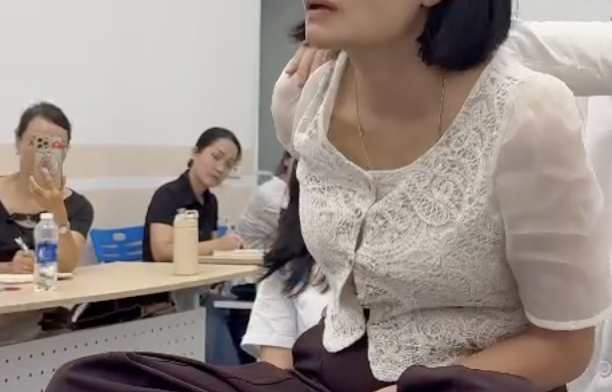
\includegraphics[width=0.48\linewidth]{xoay_mo_khop_vai_02.png}
    }
    \\ \hline
    4 & Mở khớp vai & & {%
        \hypertarget{target:mo_khop_vai}{\textbf{Mở khớp vai:}}

        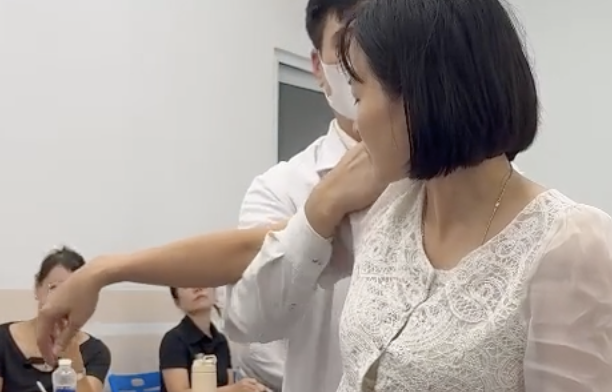
\includegraphics[width=0.48\linewidth]{mo_khp_vai.png}
        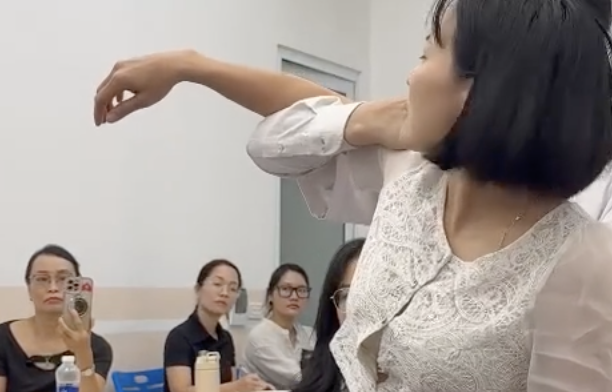
\includegraphics[width=0.48\linewidth]{mo_khop_vai_02.png}
    }
    \\ \hline
\end{longtblr}

\textbf{Vận động khuỷu tay}
\begin{longtblr}[
    caption = {Vận động khuỷu tay},
]{
    width = \textwidth,
    colspec = {|X[1,c]|X[1,c]|X[1,c]|X[9,l]|},
    % hlines,
    rowhead = 1,
}
    \hline
    STT & Tên & Số lần & Ghi chú
    \\ \hline
    1 & Gấp duỗi & 1 & {
        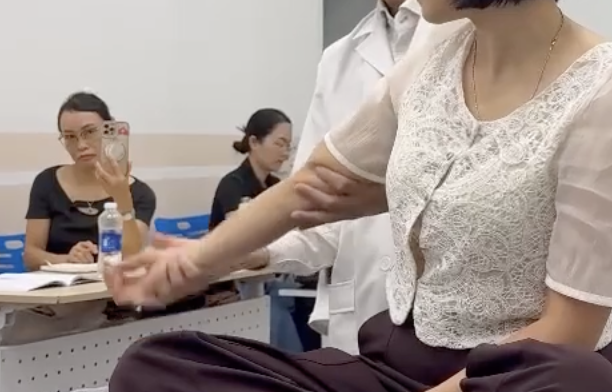
\includegraphics[width=0.48\linewidth]{khop_vai_01.png}
        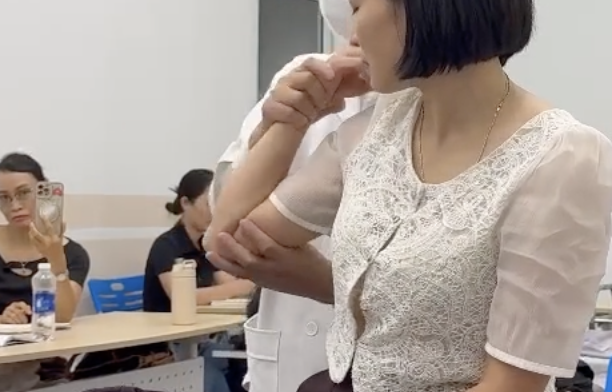
\includegraphics[width=0.48\linewidth]{khop_vai_02.png}
    }
    \\ \hline
    2 & Sấp ngửa & 1 & {
        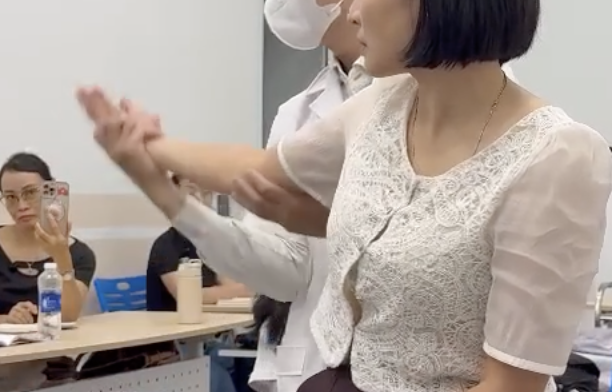
\includegraphics[width=0.48\linewidth]{sap_ngua_01.png}
        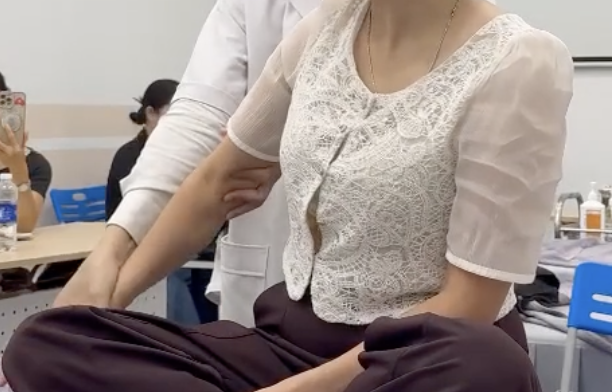
\includegraphics[width=0.48\linewidth]{sap_ngua_02.png}
    }
    \\ \hline
\end{longtblr}


\textbf{Vận động cổ tay}
\begin{longtblr}[
    caption = {Vận động cổ tay},
]{
    width = \textwidth,
    colspec = {|X[1,c]|X[1,c]|X[1,c]|X[9,l]|},
    % hlines,
    rowhead = 1,
}
    \hline
    STT & Tên & Số lần & Ghi chú
    \\ \hline
    1 & Xoay & & {
        Xoay ngược, xoay xuôi
        \newline
        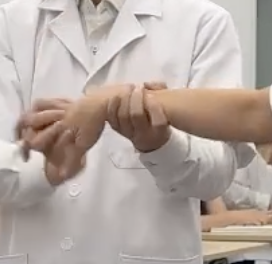
\includegraphics[width=0.48\linewidth]{xoay_co_tay_01.png}
        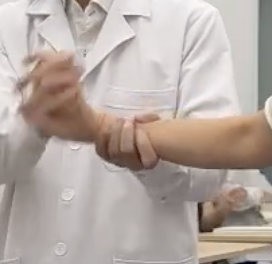
\includegraphics[width=0.48\linewidth]{xoay_co_tay_02.png}
    }
    \\ \hline
    2 & Gấp duỗi & & {
        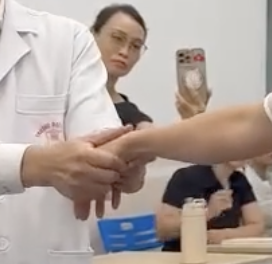
\includegraphics[width=0.48\linewidth]{gap_duoi_01.png}
        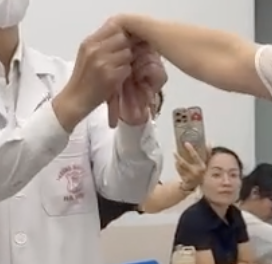
\includegraphics[width=0.48\linewidth]{gap_duoi_02.png}
        \newline
        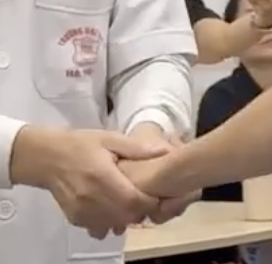
\includegraphics[width=0.48\linewidth]{gap_duoi_03.png}
        \newline
        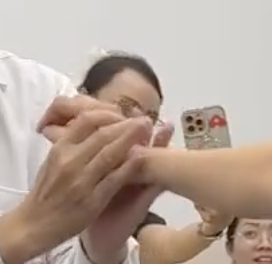
\includegraphics[width=0.48\linewidth]{duoi_01.png}
        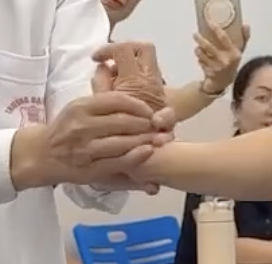
\includegraphics[width=0.48\linewidth]{duoi_02.png}
    }
    \\ \hline
\end{longtblr}

\textbf{Vận động ngón tay}
\begin{longtblr}[
    caption = {Vận đống ngón tay},
]{
    width = \textwidth,
    colspec = {|X[1,c]|X[1,c]|X[1,c]|X[9,l]|},
    % hlines,
    rowhead = 1,
}
    \hline
    STT & Tên & Số lần & Ghi chú
    \\ \hline
    1 & Vê & 5 & {
        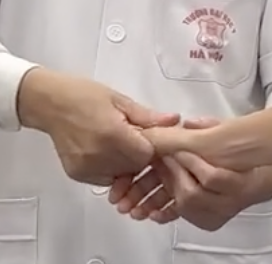
\includegraphics[width=\linewidth]{ve_ngon_tay_01.png}
    }
    \\ \hline
    2 & Vuốt & 5 & {
        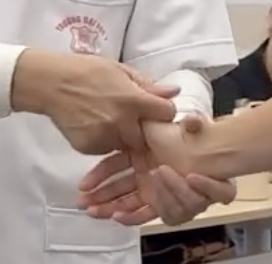
\includegraphics[width=\linewidth]{vuot_ngon_tay_01.png}
    }
    \\ \hline
\end{longtblr}


\textbf{Rung tay}
\begin{longtblr}[
    caption = {Rung tay},
]{
    width = \textwidth,
    colspec = {|X[1,c]|X[1,c]|X[1,c]|X[9,l]|},
    % hlines,
    rowhead = 1,
}
    \hline
    STT & Tên & Số lần & Ghi chú
    \\ \hline
    1 & Rung tay &  & {
    1. Bệnh nhân hơi nghiêng đối diện \newline
    2. Trước sau \newline
    3. Trên dưới \newline
    4. Kéo dãn
    \newline
    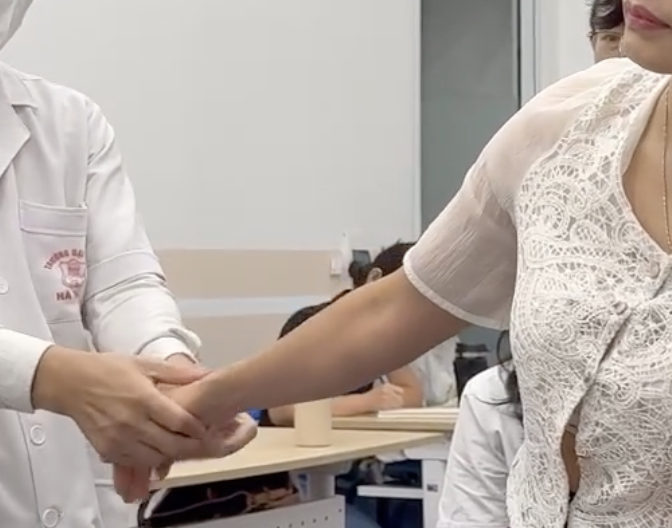
\includegraphics[width=0.48\linewidth]{rung_tay_01.png}
    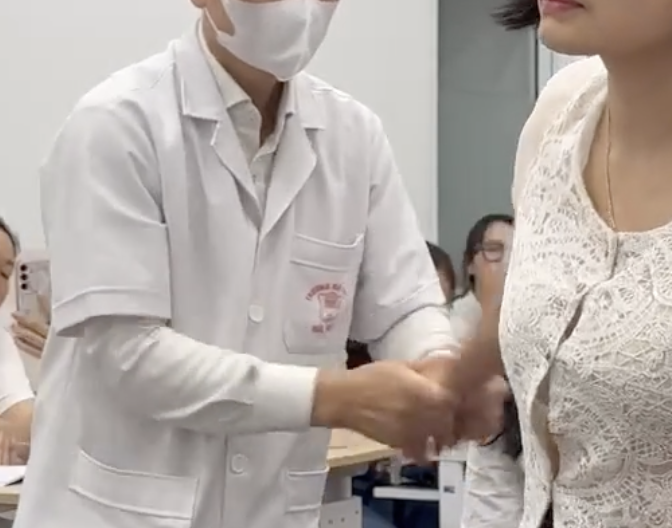
\includegraphics[width=0.48\linewidth]{rung_tay_02.png}
    \newline
    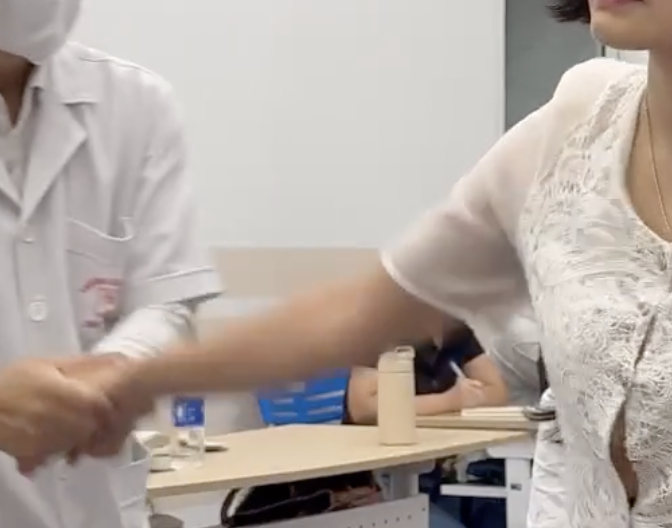
\includegraphics[width=0.48\linewidth]{rung_tay_03.png}
    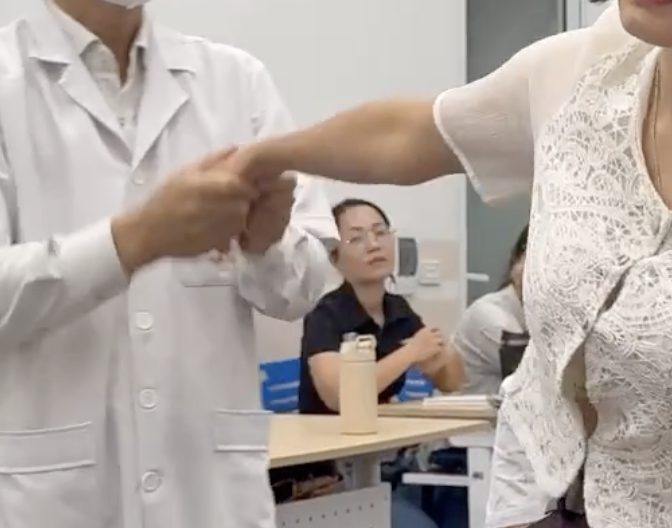
\includegraphics[width=0.48\linewidth]{rung_tay_04.png}
    \newline
    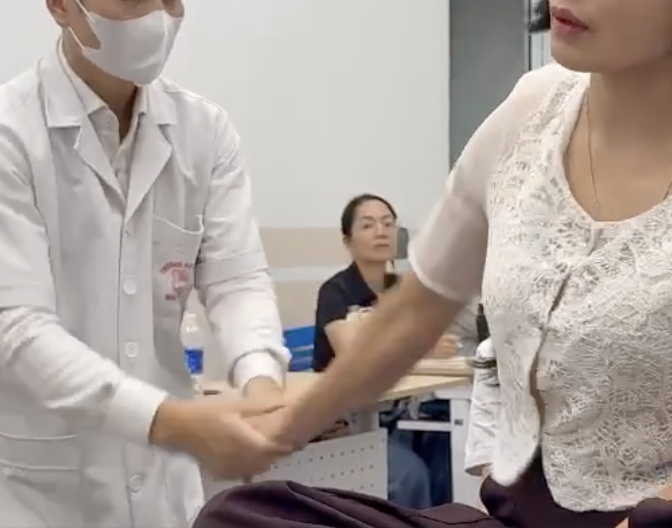
\includegraphics[width=\linewidth]{rung_tay_05.png}
    }
    \\ \hline
\end{longtblr}


\subsubsection{Vận động khớp chân}
\textbf{TƯ THẾ NẰM NGHIÊNG}

\begin{longtblr}[
    caption = {Vận động khớp tư thế nằm nghiêng},
]{
    width = \textwidth,
    colspec = {|X[1,c]|X[1,l]|X[2,l]|X[1,c]|X[7,l]|},
    % hlines,
    rowhead = 1,
}
    \hline
    STT & Tên & Vùng tác động & Số lần & Ghi chú
    \\ \hline
    1 & Vận động & Cột sống và thắt lưng cùng &  & {
        Vận động khớp cùng chậu
    
        Chi bị bệnh ở trên, thầy thuốc đứng sau người bệnh, 1 tay đặt ở khớp cùng chậu, một tay kéo giãn chi dưới và gấp nhanh chi dưới vào bụng, tay kia vẫn giữ chặt khớp cùng chậu.

        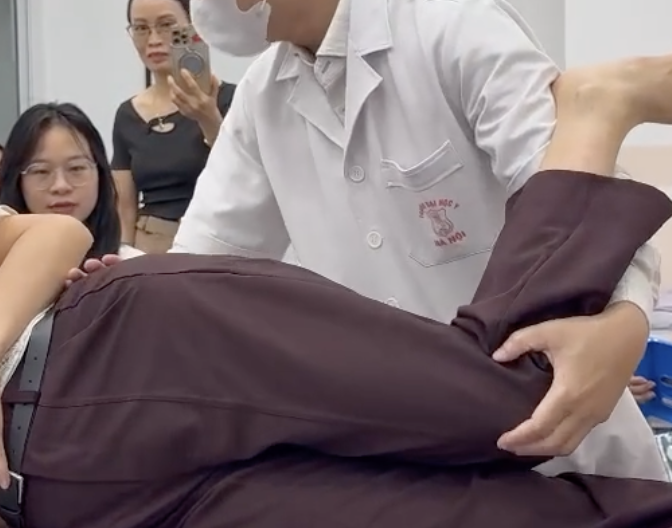
\includegraphics[width=\linewidth]{day_dau_goi_tu_the_nam_nghieng_01.png}
        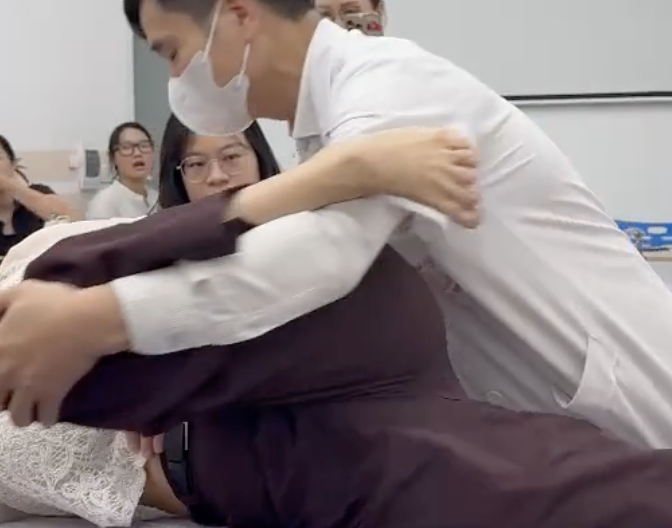
\includegraphics[width=\linewidth]{day_dau_goi_tu_the_nam_nghieng_02.png}

        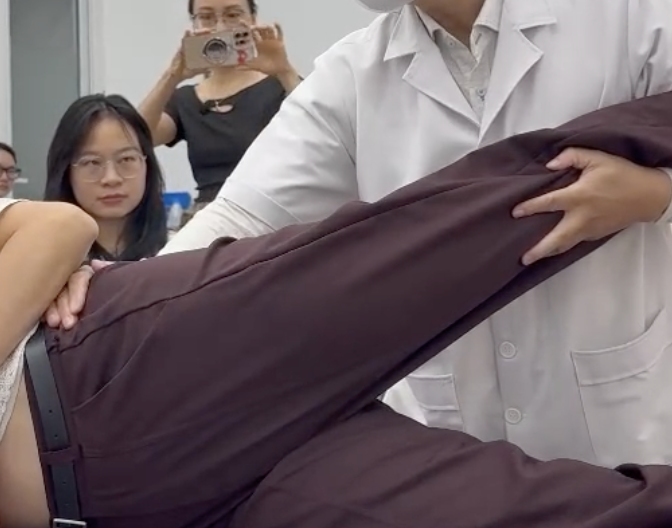
\includegraphics[width=\linewidth]{day_dau_goi_tu_the_nam_nghieng_03.png}
    }
    \\ \hline
    2 & Vận động & Cột sống và thắt lưng cùng & & {
        Vặn cột sống lưng
    
        Người bệnh nằm nghiêng, chân trên co, đầu gối để xuống giường, chân dưới duỗi, tay trên để ra sau lưng, tay dưới để tự nhiên. Thầy thuốc cùng 1 lúc 1 tay đẩy mông ra trước, 1 tay đẩy vai ra sau. Có thể nghe thấy tiếng kêu.   

        Nằm ngược lại và thực hiện tương tự.

        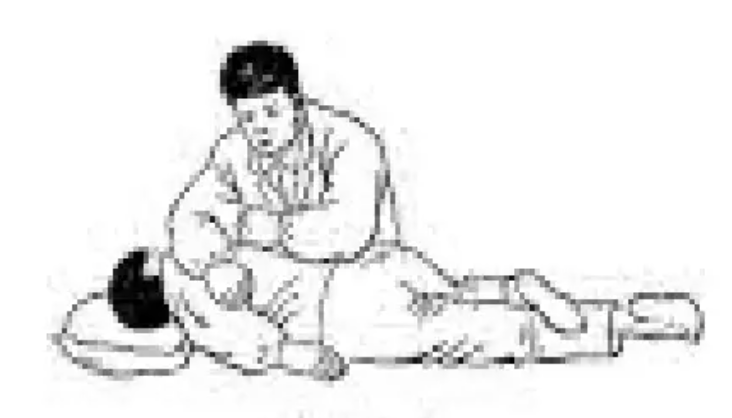
\includegraphics[width=3cm]{van_lung.png}
    }
    \\ \hline
\end{longtblr}


\textbf{TƯ THẾ NẰM NGỬA}

\begin{longtblr}[
    caption = {Vận động khớp tư thế nằm ngửa},
]{
    width = \textwidth,
    colspec = {|X[1,c]|X[1,l]|X[2,l]|X[1,c]|X[7,l]|},
    % hlines,
    rowhead = 1,
}
    \hline
    STT & Tên & Vùng tác động & Số lần & Ghi chú
    \\ \hline
    1 & Vận động & Khớp háng &  & {
        Mở khớp háng

        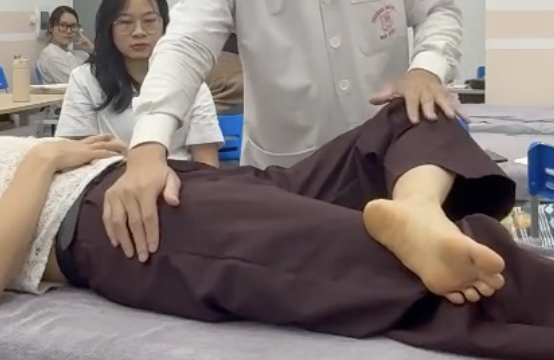
\includegraphics[width=\linewidth]{mo_khop_hang_01.png}
    }
    \\ \hline
    2 & Vận động & Khớp háng  & & {
        \hypertarget{target:van_dong_khop_hang_tu_the_nam_ngua}{\textbf{Vận động khớp háng tư thế nằm ngửa:}}

        Đẩy đầu gối
        
        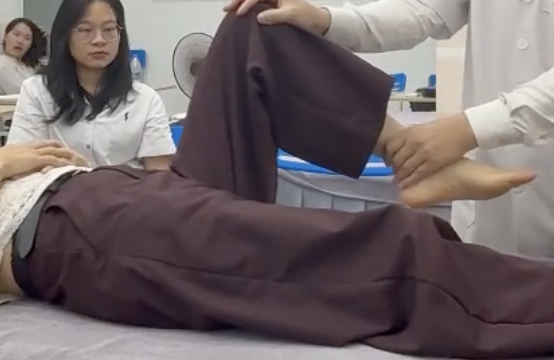
\includegraphics[width=\linewidth]{day_dau_goi_01.png}
        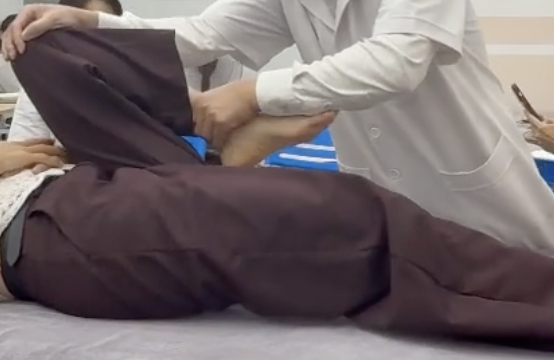
\includegraphics[width=\linewidth]{day_dau_goi_02.png}
    }
    \\ \hline
    3 & Vận động & Cột sống và khớp thắt lưng cùng & & {
        Vận động khớp cùng chậu

        \textbf{Không làm cho thoát vị đĩa đệm}
        
        Co gập chi dưới vào bụng, thầy thuốc một tay giữ chân, một tay đẩy đầu gối người bệnh sang bên phải sang bên trái 2-3 lần.

        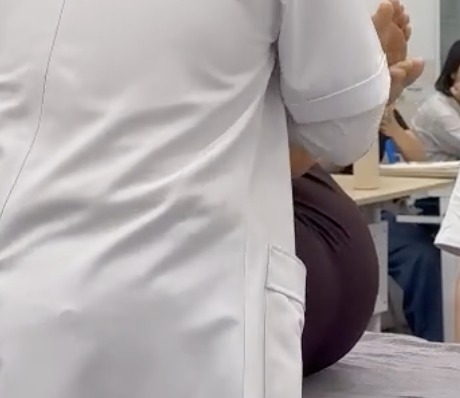
\includegraphics[width=\linewidth]{van_dong_that_lung_cung_01.png}
    }
    \\ \hline
    4 & Vận động & Cột sống và khớp thắt lưng cùng & & {
        Vận động khớp thắt lưng cùng

        Người bệnh nằm ngửa, co gập 2 chi dưới vào bụng, thầy thuốc 1 tay giữ gối, 1 tay để vào vùng cùng cụt làm cho người cong lại, rồi thả ra. 2-3 lần.

        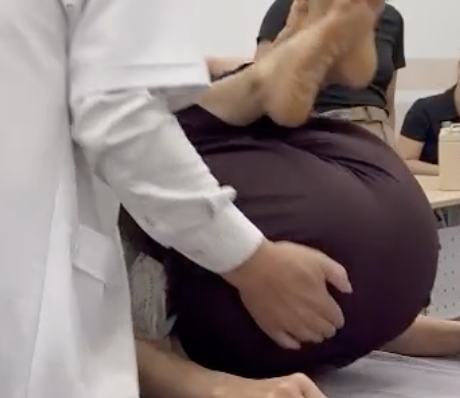
\includegraphics[width=\linewidth]{van_dong_khop_that_lung_cung_01.png}
    }
    \\ \hline
    5 & Vận động & Khớp đầu gối & & {
        Đẩy đầu gối
        \hypertarget{target:day_dau_goi}{\textbf{Đẩy đầu gối:}}

        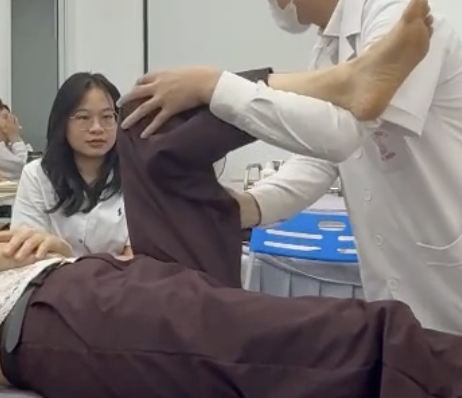
\includegraphics[width=\linewidth]{van_dong_khop_goi_01.png}
        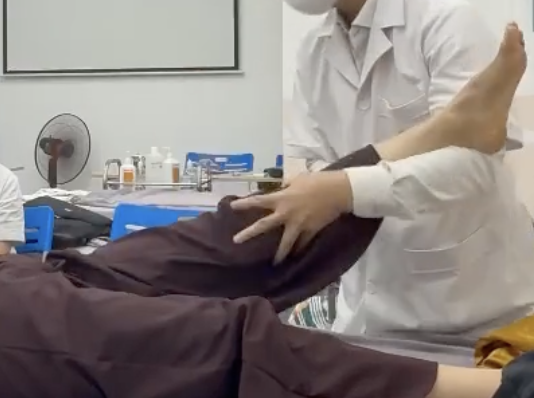
\includegraphics[width=\linewidth]{van_dong_khop_goi_02.png}
    }
    \\ \hline
    6 & Vận động & Khớp cổ chân & & {
        \hypertarget{target:xoay_co_chan}{\textbf{Xoay cổ chân:}}
    }
    \\ \hline
    7 & Vận động & Khớp cổ chân & & {
        \hypertarget{target:gap_duoi_co_chan}{\textbf{Gấp duỗi cổ chân:}}
    }
    \\ \hline
    8 & Vận động & Khớp cổ chân & & {
        \hypertarget{target:nghieng_co_chan}{\textbf{Nghiêng cổ chân:}}
    }
    \\ \hline
    9 & Vận động & Khớp ngón chân & & {
        \hypertarget{target:ve_ngon_chan}{\textbf{Vê ngón chân:}}
    }
    \\ \hline
    10 & Vận động & Khớp ngón chân & & {
        \hypertarget{target:vuot_ngon_chan}{\textbf{Vuốt ngón chân:}}
    }
    \\ \hline
\end{longtblr}

\textbf{TƯ THẾ NẰM SÂP}

\begin{longtblr}[
    caption = {Vận động khớp tư thế nằm sấp},
]{
    width = \textwidth,
    colspec = {|X[1,c]|X[1,l]|X[1,l]|X[1,c]|X[8,l]|},
    % hlines,
    rowhead = 1,
}
    \hline
    STT & Tên & Vùng tác động & Số lần & Ghi chú
    \\ \hline
    1 & Vận động &Cột sống và thắt lưng cùng (dưới) & 2-3  & {
        \noindent \textbf{Không dùng cho bệnh nhân bị thoát vị đĩa đệm.}

        Người bệnh nằm sấp, thầy thuốc 1 tay ấn lưng bệnh nhân,
         một tay nhấc 2 chân bn lên cao.

        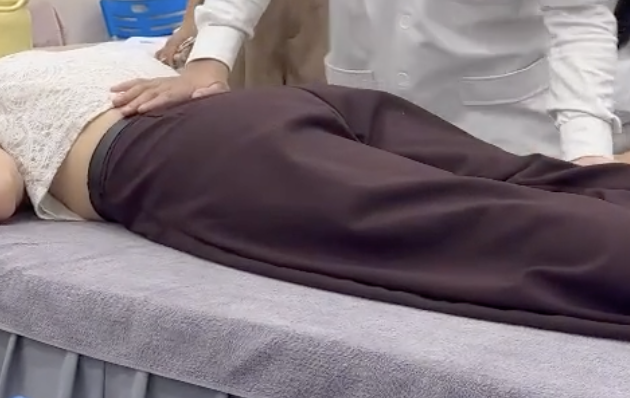
\includegraphics[width=\linewidth]{uon_lung_01.png}
        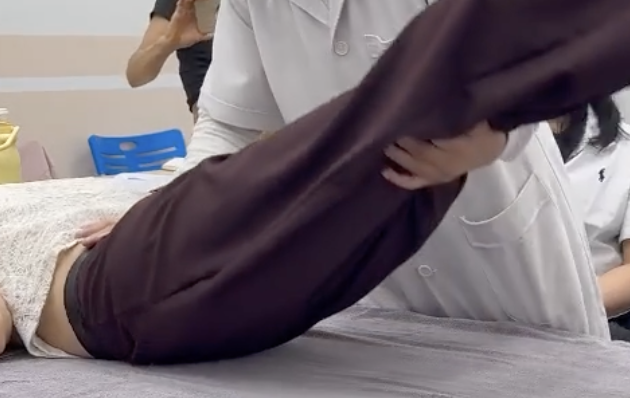
\includegraphics[width=\linewidth]{uon_lung_02.png}
    }
    \\ \hline
    2 & Vận động & Cột sống và thắt lưng cùng (trên) & 2-3 & {
        \noindent \textbf{Không dùng cho bệnh nhân bị thoát vị đĩa đệm.}

        Hai tay bệnh nhân duỗi thẳng lên đỉnh đầu.
        Người trị liệu một tay để ở giữa hai vai bệnh nhân,
        cánh tay dưới của cánh tay còn lại đỡ lấy phần trên khuỷu tay của bệnh nhân.
        Sau đó tay đẩy tay nâng thực hiện động tác.
    }
    \\ \hline
    1 & Vận động & Khớp háng & 3-5 & {
        \hypertarget{target:van_dong_khop_hang_tu_the_nam_sap}{\textbf{Vận động khớp háng tư thế nằm sấp:}}
        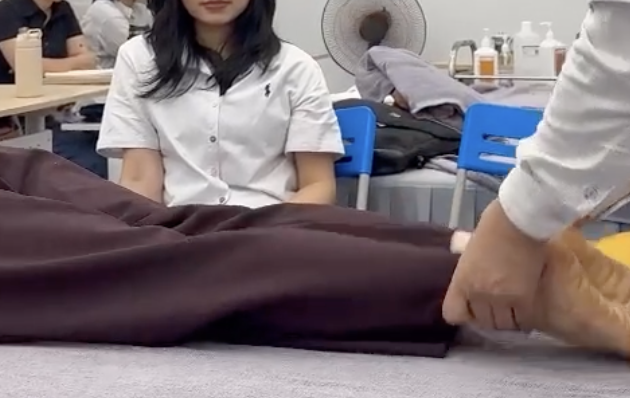
\includegraphics[width=\linewidth]{van_dong_khop_hang_tu_the_nam_sap_01.png}
        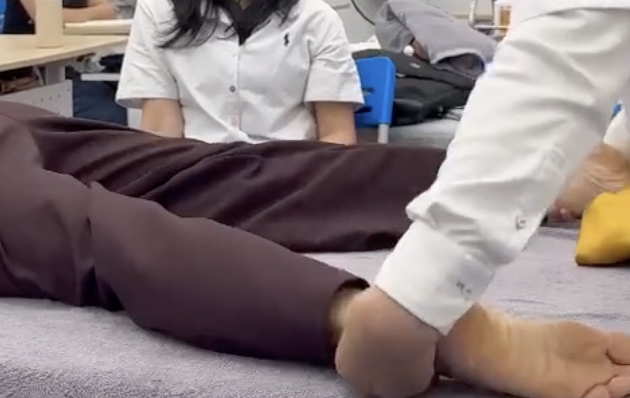
\includegraphics[width=\linewidth]{van_dong_khop_hang_tu_the_nam_sap_02.png}
    }
    \\ \hline
    1 & Vận động & Khớp gối & 3-5 & {
        \hypertarget{target:van_dong_khop_goi_tu_the_nam_sap}{\textbf{Vận động khớp gối tư thế nằm sấp:}}
        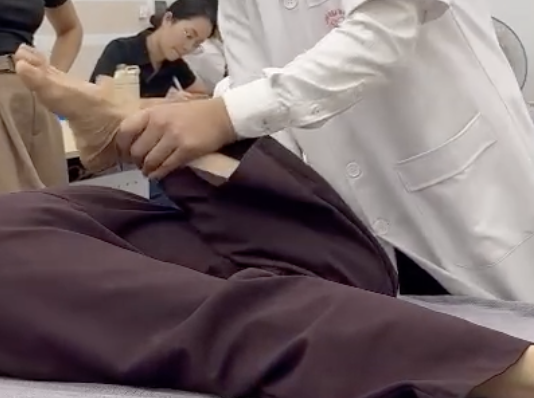
\includegraphics[width=\linewidth]{van_dong_khop_goi_tu_the_nam_sap_01.png}
        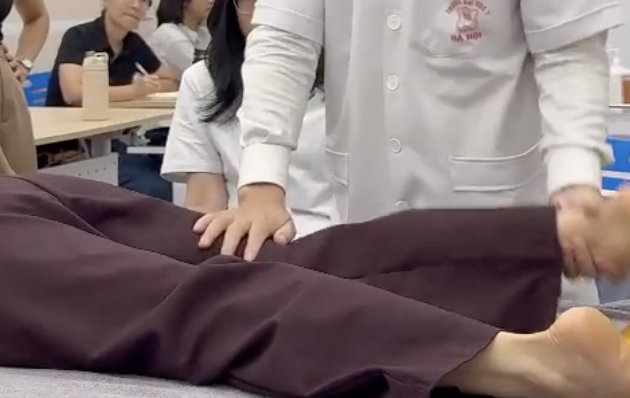
\includegraphics[width=\linewidth]{van_dong_khop_dau_goi_tu_the_nam_sap_02.png}
    }
    \\ \hline
\end{longtblr}
